\subsubsection{Uso de la aplicacion por personas sin español como idioma nativo}

{\textbf {Resumen:}}
Un usuario extranjero llega a un museo local es su ruta de turismo, al ver un cartel de la App en el museo la descarga, luego en su alojamiento decide probar la aplicación, al abrirla este se encuentra con una serie de imágenes que le muestran cómo ocupar la aplicación, estas imágenes están acompañadas de un texto en español pero el logra sin ningún problema a ocupar la aplicación.

{\textbf {Actores:}}
Usuario de nacionalidad extranjera (no chileno), Museo/Publicidad.

{\textbf {Propósito:}}
Lograr que una persona que no maneja el lenguaje nacional logre interactuar con la aplicación sin problemas, adems de demostrar su uso de manera internacional.

{\textbf {Referencias cruzadas:}}
R 1.1, R 1.2, R1.3, R3.4, R3.5

\paragraph{Caso de Uso Esencial}

\begin{longtable}{|p{5cm}|p{8cm}|}
\hline 
Acción actores & Respuesta del sistema \\ 
\hline 
El usuario llega al lugar (museo) que contiene publicidad de la aplicación. & --- \\ 
\hline 
El usuario decide descargarla y utilizarla en su casa. & --- \\ 
\hline 
El usuario inicia la aplicación. & El sistema muestra las primeras instrucciones para utilizar la cámara en conjunto con el código QR.
 \\ 
\hline 
El usuario en base a las imagenes entiende que debe apuntar con su cámara al código. & La aplicación muestra el tutorial de como desplazarse dentro de la aplicación. \\ 
\hline 
\caption{Tabla de Caso de Uso Esencial 1.2}
\label{tab22}
\end{longtable}

\paragraph{Diagrama de Caso de Uso}

\begin{figure}[H]
\centerline{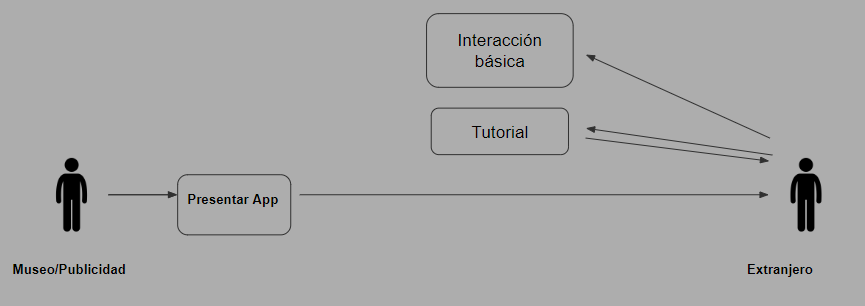
\includegraphics[width=15cm]{imgs/CasoUso_2.PNG}}
\caption{Diagrama de Caso 1.2}
\label{fig_2_1}
\end{figure}

\subsubsection{Modelo Conceptual}

\begin{figure}[H]
\centerline{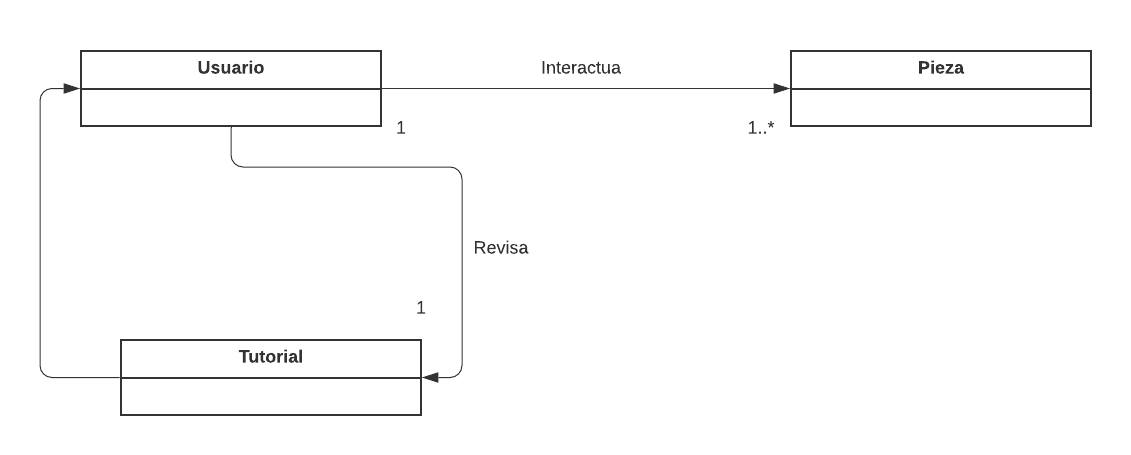
\includegraphics[width=15cm]{imgs/ModeloConceptualCaso_2_3.png}}
\caption{Modelo Conceptual Caso 1.2}
\label{fig_2_2}
\end{figure}

\paragraph{Diagrama de Secuencia o Colaboración}

\begin{figure}[H]
\centerline{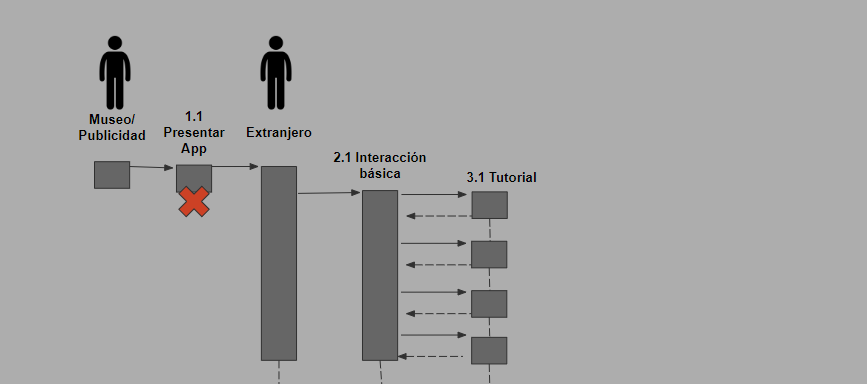
\includegraphics[width=15cm]{imgs/CasoUso_2_2.PNG}}
\caption{Diagrama de Secuencia Caso 1.2}
\label{fig_2_3}
\end{figure}

\paragraph{Priorización}
{\textbf {Tipo:}}
Relevante.